\chapter{Metodologia}

O objetivo principal deste trabalho é implementar um protótipo de um sistema VLC utilizando um SBC como plataforma de desenvolvimento. Durante o desenvolvimento elementos de metodologias ágeis, como os de \textit{Scrum} e \textit{Kanban} serão utilizados.

Para a avaliação do desempenho das SBCs selecionadas será coletado as informações de uso do processador, o uso de memória RAM e também a taxa de erros durante a transmissão de um pacote de dados.

\section{Single Board Computer (SBC)}

Single Board Computer (SBC) é um computador onde todas os componentes necessários estão em uma mesma placa de circuito impresso. Esse tipo de dispositivo é muito utilizado para fins educacionais, para desenvolvimento de sistemas, datacenters (centros  de  processamento  de  dados) e clusters portáteis. Alguns exemplos são o \textit{OrangePI}, \textit{RockPI}, \textit{BeagleBone} e \textit{RaspberryPI}, sendo este um dos mais populares \cite{SBC_edu}.

Os SBCs geralmente são de baixo custo, porém devido a escassez global de semicondutores reduziu a sua disponibilidade e por consequência levou ao aumento dos preços \cite{zeng_2022}. Principalmente do \textit{RaspberryPI} que passou de 45 dólares para 161 dólares, por esse motivo o SBC \textit{OrangePI} foi selecionado para o desenvolvimento deste trabalho.

\subsection{RaspberryPI}

A \textit{Raspberry Pi Foundation} foi fundada em 2008 sediada no Reino Unido com o objetivo de promover o avanço na educação no campo da computação. \cite{rasp}

O \textit{RaspberryPI} é um pequeno computador que traz consigo um processador na arquitetura ARM, a mesma tecnologia que encontra num smartphone \cite{rasp}.

\begin{figure}[!htbp]
  \caption{Raspberry Pi 3}
  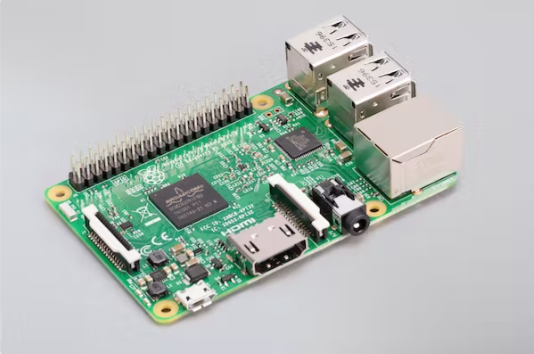
\includegraphics[scale=0.4]{images/rasp.png}
  \legend{Fonte: \citeauthor{rasp}}
  \label{figura:rasp}
\end{figure}

\subsection{OrangePI}

O \textit{OrangePI} é um produto \textit{open source} focado em entregar hardware de baixo custo. A arquitetura de seu processador é ARM e a plataforma suporta vários sistemas operacionais como Android e as varias distribuições de linux \cite{orangepi}.

\begin{figure}[!htbp]
  \caption{Orange Pi 3 LTS}
  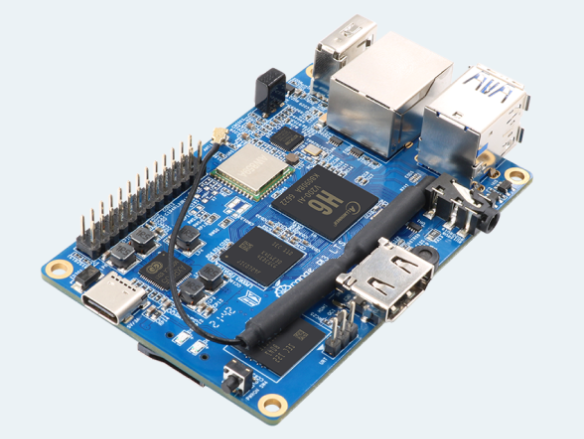
\includegraphics[scale=0.4]{images/orange.png}
  \legend{Fonte: \citeauthor{orangepi}}
  \label{figura:orange}
\end{figure}

